\documentclass[]{article}
\usepackage{lmodern}
\usepackage{amssymb,amsmath}
\usepackage{ifxetex,ifluatex}
\usepackage{fixltx2e} % provides \textsubscript
\ifnum 0\ifxetex 1\fi\ifluatex 1\fi=0 % if pdftex
  \usepackage[T1]{fontenc}
  \usepackage[utf8]{inputenc}
\else % if luatex or xelatex
  \ifxetex
    \usepackage{mathspec}
  \else
    \usepackage{fontspec}
  \fi
  \defaultfontfeatures{Ligatures=TeX,Scale=MatchLowercase}
\fi
% use upquote if available, for straight quotes in verbatim environments
\IfFileExists{upquote.sty}{\usepackage{upquote}}{}
% use microtype if available
\IfFileExists{microtype.sty}{%
\usepackage{microtype}
\UseMicrotypeSet[protrusion]{basicmath} % disable protrusion for tt fonts
}{}
\usepackage[margin=1in]{geometry}
\usepackage{hyperref}
\hypersetup{unicode=true,
            pdftitle={Homework 7},
            pdfauthor={Christophe Hunt},
            pdfborder={0 0 0},
            breaklinks=true}
\urlstyle{same}  % don't use monospace font for urls
\usepackage{color}
\usepackage{fancyvrb}
\newcommand{\VerbBar}{|}
\newcommand{\VERB}{\Verb[commandchars=\\\{\}]}
\DefineVerbatimEnvironment{Highlighting}{Verbatim}{commandchars=\\\{\}}
% Add ',fontsize=\small' for more characters per line
\usepackage{framed}
\definecolor{shadecolor}{RGB}{248,248,248}
\newenvironment{Shaded}{\begin{snugshade}}{\end{snugshade}}
\newcommand{\KeywordTok}[1]{\textcolor[rgb]{0.13,0.29,0.53}{\textbf{{#1}}}}
\newcommand{\DataTypeTok}[1]{\textcolor[rgb]{0.13,0.29,0.53}{{#1}}}
\newcommand{\DecValTok}[1]{\textcolor[rgb]{0.00,0.00,0.81}{{#1}}}
\newcommand{\BaseNTok}[1]{\textcolor[rgb]{0.00,0.00,0.81}{{#1}}}
\newcommand{\FloatTok}[1]{\textcolor[rgb]{0.00,0.00,0.81}{{#1}}}
\newcommand{\ConstantTok}[1]{\textcolor[rgb]{0.00,0.00,0.00}{{#1}}}
\newcommand{\CharTok}[1]{\textcolor[rgb]{0.31,0.60,0.02}{{#1}}}
\newcommand{\SpecialCharTok}[1]{\textcolor[rgb]{0.00,0.00,0.00}{{#1}}}
\newcommand{\StringTok}[1]{\textcolor[rgb]{0.31,0.60,0.02}{{#1}}}
\newcommand{\VerbatimStringTok}[1]{\textcolor[rgb]{0.31,0.60,0.02}{{#1}}}
\newcommand{\SpecialStringTok}[1]{\textcolor[rgb]{0.31,0.60,0.02}{{#1}}}
\newcommand{\ImportTok}[1]{{#1}}
\newcommand{\CommentTok}[1]{\textcolor[rgb]{0.56,0.35,0.01}{\textit{{#1}}}}
\newcommand{\DocumentationTok}[1]{\textcolor[rgb]{0.56,0.35,0.01}{\textbf{\textit{{#1}}}}}
\newcommand{\AnnotationTok}[1]{\textcolor[rgb]{0.56,0.35,0.01}{\textbf{\textit{{#1}}}}}
\newcommand{\CommentVarTok}[1]{\textcolor[rgb]{0.56,0.35,0.01}{\textbf{\textit{{#1}}}}}
\newcommand{\OtherTok}[1]{\textcolor[rgb]{0.56,0.35,0.01}{{#1}}}
\newcommand{\FunctionTok}[1]{\textcolor[rgb]{0.00,0.00,0.00}{{#1}}}
\newcommand{\VariableTok}[1]{\textcolor[rgb]{0.00,0.00,0.00}{{#1}}}
\newcommand{\ControlFlowTok}[1]{\textcolor[rgb]{0.13,0.29,0.53}{\textbf{{#1}}}}
\newcommand{\OperatorTok}[1]{\textcolor[rgb]{0.81,0.36,0.00}{\textbf{{#1}}}}
\newcommand{\BuiltInTok}[1]{{#1}}
\newcommand{\ExtensionTok}[1]{{#1}}
\newcommand{\PreprocessorTok}[1]{\textcolor[rgb]{0.56,0.35,0.01}{\textit{{#1}}}}
\newcommand{\AttributeTok}[1]{\textcolor[rgb]{0.77,0.63,0.00}{{#1}}}
\newcommand{\RegionMarkerTok}[1]{{#1}}
\newcommand{\InformationTok}[1]{\textcolor[rgb]{0.56,0.35,0.01}{\textbf{\textit{{#1}}}}}
\newcommand{\WarningTok}[1]{\textcolor[rgb]{0.56,0.35,0.01}{\textbf{\textit{{#1}}}}}
\newcommand{\AlertTok}[1]{\textcolor[rgb]{0.94,0.16,0.16}{{#1}}}
\newcommand{\ErrorTok}[1]{\textcolor[rgb]{0.64,0.00,0.00}{\textbf{{#1}}}}
\newcommand{\NormalTok}[1]{{#1}}
\usepackage{graphicx,grffile}
\makeatletter
\def\maxwidth{\ifdim\Gin@nat@width>\linewidth\linewidth\else\Gin@nat@width\fi}
\def\maxheight{\ifdim\Gin@nat@height>\textheight\textheight\else\Gin@nat@height\fi}
\makeatother
% Scale images if necessary, so that they will not overflow the page
% margins by default, and it is still possible to overwrite the defaults
% using explicit options in \includegraphics[width, height, ...]{}
\setkeys{Gin}{width=\maxwidth,height=\maxheight,keepaspectratio}
\IfFileExists{parskip.sty}{%
\usepackage{parskip}
}{% else
\setlength{\parindent}{0pt}
\setlength{\parskip}{6pt plus 2pt minus 1pt}
}
\setlength{\emergencystretch}{3em}  % prevent overfull lines
\providecommand{\tightlist}{%
  \setlength{\itemsep}{0pt}\setlength{\parskip}{0pt}}
\setcounter{secnumdepth}{5}
% Redefines (sub)paragraphs to behave more like sections
\ifx\paragraph\undefined\else
\let\oldparagraph\paragraph
\renewcommand{\paragraph}[1]{\oldparagraph{#1}\mbox{}}
\fi
\ifx\subparagraph\undefined\else
\let\oldsubparagraph\subparagraph
\renewcommand{\subparagraph}[1]{\oldsubparagraph{#1}\mbox{}}
\fi

%%% Use protect on footnotes to avoid problems with footnotes in titles
\let\rmarkdownfootnote\footnote%
\def\footnote{\protect\rmarkdownfootnote}

%%% Change title format to be more compact
\usepackage{titling}

% Create subtitle command for use in maketitle
\newcommand{\subtitle}[1]{
  \posttitle{
    \begin{center}\large#1\end{center}
    }
}

\setlength{\droptitle}{-2em}
  \title{Homework 7}
  \pretitle{\vspace{\droptitle}\centering\huge}
  \posttitle{\par}
  \author{Christophe Hunt}
  \preauthor{\centering\large\emph}
  \postauthor{\par}
  \predate{\centering\large\emph}
  \postdate{\par}
  \date{March 18, 2017}

\usepackage{relsize}
\usepackage{setspace}
\usepackage{amsmath,amsfonts,amsthm}
\usepackage[sfdefault]{roboto}
\usepackage[T1]{fontenc}
\usepackage{float}
\usepackage{multirow}
\usepackage{mathtools}

\begin{document}
\maketitle

{
\setcounter{tocdepth}{2}
\tableofcontents
}
\newpage

\section{Page 304: problem 2}\label{page-304-problem-2}

The bridges and land masses of a certain city can be modeled with graph
G in figure 8.7.

\begin{figure}[htbp]
\centering
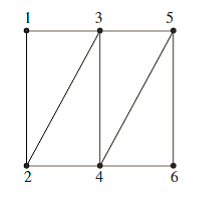
\includegraphics{https://raw.githubusercontent.com/ChristopheHunt/MSDA---Coursework/master/Data\%20609/Homework\%207/bridges.PNG}
\caption{}
\end{figure}

\subsection{a. is G Eularian? Why or why
not?}\label{a.-is-g-eularian-why-or-why-not}

\begin{quote}
No, because there are vertices of odd degrees (2 and 5).
\end{quote}

\subsection{b. Suppose we relax the requirement of the walk so that the
walker need not start and end at the same land mass but still must
traverse every bridge exactly once. Is this type of walk possible in a
city modeled by the graph in figure 8.7? If so, how? If not, why
not?}\label{b.-suppose-we-relax-the-requirement-of-the-walk-so-that-the-walker-need-not-start-and-end-at-the-same-land-mass-but-still-must-traverse-every-bridge-exactly-once.-is-this-type-of-walk-possible-in-a-city-modeled-by-the-graph-in-figure-8.7-if-so-how-if-not-why-not}

\begin{quote}
Yes, it is possible to travese each edge once.\\
We can start our walk at 2 and then traverse as follows:\\
1. 2 to 1\\
2. 1 to 3\\
3. 3 to 2\\
4. 2 to 4\\
5. 4 to 5\\
6. 5 to 3\\
7. 3 to 4\\
8. 4 to 6\\
9. 6 to 5
\end{quote}

\newpage

\section{Page 307: problem 1}\label{page-307-problem-1}

Consider the graph in Figure 8.11.

\subsection{a. Write down the set of edges
E(G)}\label{a.-write-down-the-set-of-edges-eg}

\begin{quote}
\(E(G) = \{ab, ae, af, bc, bd, cd, de, df, ef\}\)
\end{quote}

\subsection{b. Which edges are incident with vertex
b?}\label{b.-which-edges-are-incident-with-vertex-b}

\begin{quote}
ab, bc, and bd
\end{quote}

\subsection{c. Which vertices are adjacent to vertex
c?}\label{c.-which-vertices-are-adjacent-to-vertex-c}

\begin{quote}
b and d
\end{quote}

\subsection{d. Compute deg(a)}\label{d.-compute-dega}

\begin{quote}
deg(a) = \{ab, ae, af\} = 3
\end{quote}

\subsection{\texorpdfstring{e. Compute
\(|E(G)|\)}{e. Compute \textbar{}E(G)\textbar{}}}\label{e.-compute-eg}

\begin{quote}
\(|E(G)|= \{ab, ae, af, bc, bd, cd, de, df, ef\} = 9\)
\end{quote}

\newpage

\section{Page 320: problem 10}\label{page-320-problem-10}

A basketball coach needs to find a starting lineup for her team. There
are five positions that must be filled: point guard (1), shooting guard
(2), swing(3), power forward (4), and center (5). Given the Table 8.7,
create a graph model and use it to find a feasible starting lineup. What
changes if the coach decides she cant play Hermione in position 3?

\begin{Shaded}
\begin{Highlighting}[]
\KeywordTok{library}\NormalTok{(igraph)}
\end{Highlighting}
\end{Shaded}

\begin{Shaded}
\begin{Highlighting}[]
\NormalTok{b_team <-}\StringTok{ }\KeywordTok{data.frame}\NormalTok{(}\DataTypeTok{from =} \KeywordTok{c}\NormalTok{(}\StringTok{'Alice'}\NormalTok{,}\StringTok{'Alice'}\NormalTok{,}
                                 \StringTok{'Bonnie'}\NormalTok{, }
                                 \StringTok{'Courtney'}\NormalTok{, }\StringTok{'Courtney'}\NormalTok{, }
                                 \StringTok{'Deb'}\NormalTok{,  }\StringTok{'Deb'}\NormalTok{,  }\StringTok{'Deb'}\NormalTok{,}
                                 \StringTok{'Ellen'}\NormalTok{, }
                                 \StringTok{'Fay'}\NormalTok{,}
                                 \StringTok{'Gladys'}\NormalTok{, }\StringTok{'Gladys'}\NormalTok{,}
                                 \StringTok{'Hermione'}\NormalTok{, }\StringTok{'Hermione'}\NormalTok{),}
                        
                        \DataTypeTok{to =} \KeywordTok{c}\NormalTok{(}\StringTok{'point guard (1)'}\NormalTok{,}\StringTok{'shooting guard (2)'}\NormalTok{,}
                               \StringTok{'point guard (1)'}\NormalTok{,}
                               \StringTok{'point guard (1)'}\NormalTok{,}\StringTok{'shooting guard (2)'}\NormalTok{,}
                               \StringTok{'swing (3)'}\NormalTok{, }\StringTok{'power forward (4)'}\NormalTok{, }\StringTok{'center (5)'}\NormalTok{,}
                               \StringTok{'shooting guard (2)'}\NormalTok{,}
                               \StringTok{'point guard (1)'}\NormalTok{,}
                               \StringTok{'swing (3)'}\NormalTok{, }\StringTok{'power forward (4)'}\NormalTok{,}
                               \StringTok{'point guard (1)'}\NormalTok{, }\StringTok{'swing (3)'}\NormalTok{),}
                        \DataTypeTok{weight =} \KeywordTok{c}\NormalTok{(}\DecValTok{1}\NormalTok{,}\DecValTok{1}\NormalTok{,}\DecValTok{1}\NormalTok{,}\DecValTok{1}\NormalTok{,}\DecValTok{1}\NormalTok{,}\DecValTok{1}\NormalTok{,}\DecValTok{1}\NormalTok{,}\DecValTok{1}\NormalTok{,}\DecValTok{1}\NormalTok{,}\DecValTok{1}\NormalTok{,}\DecValTok{1}\NormalTok{,}\DecValTok{1}\NormalTok{,}\DecValTok{1}\NormalTok{,}\DecValTok{1} \NormalTok{))}

\NormalTok{df_b_team <-}\StringTok{ }\KeywordTok{graph.data.frame}\NormalTok{(b_team, }\DataTypeTok{directed=}\OtherTok{FALSE}\NormalTok{)}
\KeywordTok{plot}\NormalTok{(df_b_team,}\DataTypeTok{vertex.color=}\StringTok{"gold"}\NormalTok{, }
     \DataTypeTok{vertex.size=}\DecValTok{6}\NormalTok{, }
     \DataTypeTok{asp =} \NormalTok{.}\DecValTok{7}\NormalTok{,}
     \DataTypeTok{vertex.frame.color=}\StringTok{"gray"}\NormalTok{, }
     \DataTypeTok{vertex.label.color=}\StringTok{"black"}\NormalTok{,  }
     \DataTypeTok{edge.curved=}\FloatTok{0.2}\NormalTok{)}
\end{Highlighting}
\end{Shaded}

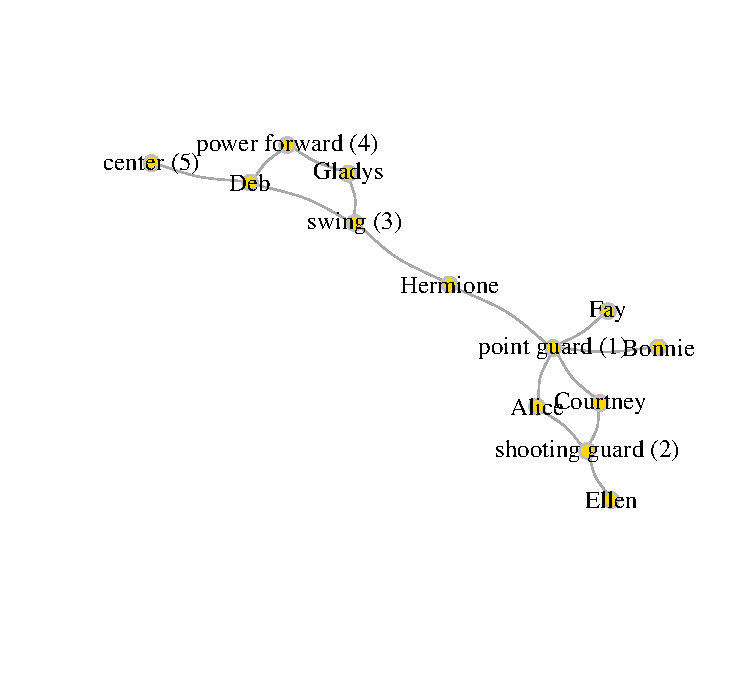
\includegraphics{Christophe_Hunt_hw7_files/figure-latex/unnamed-chunk-2-1.pdf}

\begin{quote}
Using the graph, we can see that a possible lineup is:\\
Ellen - Shooting Guard\\
Fay - Point Guard\\
Hermione - Swing\\
Gladys - Power Forward\\
Deb - Center
\end{quote}

\begin{quote}
If the coach decides she can't play Hermione in position 3 swing, she
wont be able to fill the lineup. This is because Deb and Gladys are the
only others that can play position 3 but they also are the only ones
that can play other positions.
\end{quote}

\newpage

\section{Page 331: problem 1}\label{page-331-problem-1}

Find a shortest path from node \(a\) to node \(j4\) in the graph in
Figure 8.33 with edge weights shown on the graph.

\begin{figure}[htbp]
\centering
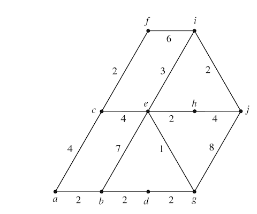
\includegraphics{https://raw.githubusercontent.com/ChristopheHunt/MSDA---Coursework/master/Data\%20609/Homework\%207/problem1.PNG}
\caption{}
\end{figure}

\begin{Shaded}
\begin{Highlighting}[]
\NormalTok{path <-}\StringTok{ }\KeywordTok{data.frame}\NormalTok{(}\DataTypeTok{from=}\KeywordTok{c}\NormalTok{(}\StringTok{'a'}\NormalTok{,}\StringTok{'a'}\NormalTok{,}\StringTok{'b'}\NormalTok{,}\StringTok{'b'}\NormalTok{,}\StringTok{'c'}\NormalTok{,}\StringTok{'c'}\NormalTok{,}
                          \StringTok{'d'}\NormalTok{,}\StringTok{'e'}\NormalTok{,}\StringTok{'g'}\NormalTok{,}\StringTok{'f'}\NormalTok{,}\StringTok{'i'}\NormalTok{,}\StringTok{'e'}\NormalTok{,}
                          \StringTok{'h'}\NormalTok{, }\StringTok{'e'}\NormalTok{),}
                   \DataTypeTok{to =}\KeywordTok{c}\NormalTok{(}\StringTok{'b'}\NormalTok{,}\StringTok{'c'}\NormalTok{,}\StringTok{'e'}\NormalTok{,}\StringTok{'d'}\NormalTok{,}\StringTok{'e'}\NormalTok{,}\StringTok{'f'}\NormalTok{,}
                         \StringTok{'g'}\NormalTok{,}\StringTok{'g'}\NormalTok{,}\StringTok{'i'}\NormalTok{,}\StringTok{'i'}\NormalTok{,}\StringTok{'j'}\NormalTok{,}\StringTok{'h'}\NormalTok{,}
                         \StringTok{'j'}\NormalTok{,}\StringTok{'i'}\NormalTok{),}
                        \DataTypeTok{weight =} \KeywordTok{c}\NormalTok{(}\DecValTok{2}\NormalTok{,}\DecValTok{4}\NormalTok{,}\DecValTok{7}\NormalTok{,}\DecValTok{2}\NormalTok{,}\DecValTok{4}\NormalTok{,}\DecValTok{2}\NormalTok{,}
                                   \DecValTok{2}\NormalTok{,}\DecValTok{1}\NormalTok{,}\DecValTok{8}\NormalTok{,}\DecValTok{6}\NormalTok{,}\DecValTok{2}\NormalTok{,}\DecValTok{2}\NormalTok{,}
                                   \DecValTok{4}\NormalTok{,}\DecValTok{3}\NormalTok{))}

\NormalTok{g <-}\StringTok{ }\KeywordTok{graph.data.frame}\NormalTok{(path, }\DataTypeTok{directed=}\OtherTok{FALSE}\NormalTok{)}

\NormalTok{path_length <-}\StringTok{ }\KeywordTok{shortest.paths}\NormalTok{(g, }\DataTypeTok{v =} \StringTok{'a'}\NormalTok{, }\DataTypeTok{to =} \StringTok{'j'}\NormalTok{)}

\NormalTok{path_output <-}\StringTok{ }\KeywordTok{get.shortest.paths}\NormalTok{(g, }\StringTok{'a'}\NormalTok{, }\StringTok{'j'}\NormalTok{)}

\NormalTok{path_output$vpath[[}\DecValTok{1}\NormalTok{]]}
\end{Highlighting}
\end{Shaded}

\begin{verbatim}
## + 7/10 vertices, named:
## [1] a b d g e i j
\end{verbatim}

The shortest path is 12 and the path is (a b d g e i j).


\end{document}
